%! Author = cnatzke
%! Date = 05/24/2022
\documentclass[cnatzke_thesis_proposal.tex]{subfiles}
\usepackage{amssymb}
\begin{document}

%------------------------------------------
\subsection{Nuclear Equation of State}
%------------------------------------------
The Nuclear Equation of State (EOS) governs the properties of nuclear matter and defines the characteristics of neutron-rich nuclei, the structure of neutron stars, supernova explosions and compact object mergers \cite{knupfer_scaling_1985}. 
The EOS is well constrained for symmetric nuclear matter, matter where the number of protons and neutrons are roughly equal, but the properties for asymmetric, neutron rich matter require further investigation \cite{danielewicz_determination_2002}.
The largest uncertainties in the EOS for neutron rich matter lie in the limited knowledge of the symmetry energy $J$, the difference between the energies of neutron and nuclear matter at saturation density, and the slope of the symmetry energy $L$, which governs the pressure of neutron matter. 

Atomic nuclei provide a terrestrial probe of nuclear matter and the symmetry energy $J$, where it contributes to the formation of neutron skins in systems with a neutron excess. 
$J$ and $L$ can be correlated with isovector collective excitations of nucleus, such as the pygmy dipole resonance \cite{carbone_constraints_2010} and giant dipole resonances (GDRs) \cite{trippa_giant_2008}, via calulations based on energy density functionals (EDFs) suggesting the neutron skin thickness, the difference between the point-neutron and point-proton radii~\cite{tsang_constraints_2012}, could be constrained by measuring isovector collective observables at low energy \cite{krasznahorkay_excitation_1999}.
A direct experimental measurement of $R_{skin}$ is extremely challenging but can be indirectly extracted by its correlation to collective isovector observables at low energies \cite{birkhan_electric_2017}. 
One such observable is the dipole polarizability $\alpha_D$ \cite{birkhan_electric_2017}, providing an experimentally viable tool to constrain the EOS of neutron matter and the physics of neutron stars. 
% TODO : Add citations to last sentence. 6-11 from birkham

%------------------------------------------
\subsection{Electric Polarizability and Magnetic Susceptibility}
%------------------------------------------
Polarizability is a fundamental concept in physics that describes how applied electric or magnetic fields induce an electric or magnetic multipole moment in the matter of interest \cite{jackson_classical_1999} and plays a large role in nuclear physics observables.
In fact, DFT calculations suggest a strong correlation between the static dipole polarizability, $\alpha_D$, and the neutron radius, $R_{n}$~\cite{hagen_neutron_2016}. 
The static dipole polarization of the ground and excited state shape of atomic nuclei is influenced by the state's coupling to higher-energy collective modes, like the GDR and pygmy dipole resonance, via virtual excitations. 
As described in Ref.~\cite{soderstrom_electromagnetic_2020}, $\alpha_D$ can be obtained from the photonuclear population of excited states, given by

\begin{equation} \label{eqn:scalar_dipole_polarizability}
    \alpha_{D,E1} = 2 e \sum_n \frac{|\langle I_0 || E1 || I_n \rangle |^2}{E_n - E_0}
\end{equation}

where $I_0$, $E1$, and $I_n$ are the matrix elements for the ground state, electric dipole transition, and excited state respectively; $e$ is the elementary charge of the electron; and $E_n$ is the energy of the state. 
The value of $\alpha_D$, and the analogous magnetic susceptibility $\chi$, in atomic and nuclear systems spans many orders of magnitude depending on the scale of interest, for example the magnetic susceptibility of a nucleus is twelve orders of magnitude smaller than that of an atom \cite{knupfer_scaling_1985}.

The polarizability can be expanded past the scalar case to include separate tensor components describing higher-order electric and magnetic multipoles~\cite{soderstrom_electromagnetic_2020}. 
Using the nuclear structure framework these off diagonal polarizabilities appear as very weak second-order electromagnetic processes that can be expressed analogously to Eq. (\ref{eqn:scalar_dipole_polarizability}) in terms of either electric and magnetic components or different multipolarities. 

\begin{equation} \label{eqn:m2e2_dipole_polarizability}
    \alpha_{M2E2} = \sum_n \frac{\langle I_f || E2 || I_n \rangle \langle I_n || M2 || I_i \rangle}{E_n - \omega}
\end{equation}

or 

\begin{equation} \label{eqn:m2e2_dipole_polarizability}
    \alpha_{E3M1} = \sum_n \frac{\langle I_f || M1 || I_n \rangle \langle I_n || E3 || I_i \rangle}{E_n - \omega}
\end{equation}

where $\omega$ is the interference frequency of the emitted gamma-rays and is approximated to one half of the initial energy. 
This second-order electromagnetic process was discussed in the doctorate dissertation of Maria G\"oppert-Mayer~\cite{goppert-mayer_uber_1931} where the estimated relative probability of two-photon absorption to the single-photon process is $10^{-7}$. 

The electric dipole polarizability has been measured for a variety of stable isotopes, $^{48}$Ca \cite{birkhan_electric_2017}, $^{120}$Sn \cite{hashimoto_dipole_2015}, and $^{208}$Pb \cite{tamii_complete_2011} using proton inelastic scattering, and $\alpha_D$ has only been measured for one short-lived nucleus, $^{68}$Ni~\cite{rossi_measurement_2013}.
At this time the electric dipole polarizability for a short-lived nuclear state has not been experimentally measured, but using the \textit{transition} electric polarizability, the difference in $\alpha_D$ between the two states, and the ground state polarizability the polarizability of a short-lived nuclear state can be measured.
This proposal highlights work towards the first measurement of this quantity using nuclear two-photon decay which is a uniquely suited probe of the transition polarizability.

%------------------------------------------
\subsection{Nuclear Gamma Decay and Internal Conversion}
%------------------------------------------
Nuclear gamma decay is an electromagnetic process in which an unstable nucleus deexcites into a more energetically favourable state via the emission of a photon.
The energy of the photon is roughly equivalent to the energy difference in the initial and final states of the nucleus (save for a small amount of recoil kinetic energy imparted to the nucleus) and the photon's angular momentum equals the difference in angular momentum of the nucleus' state. 
This restriction on angular momentum forbids the emission of a $\gamma$-ray from two states $0^+$ states since the photon is a spin 0 Boson and cannot carry away less than $1\hbar$ units of angular momentum. 

Gamma-decay often competes with another first-order decay mode called Internal Conversion (IC) which is an electroweak process where the nucleus deexcites by transferring its energy to an atomic electron. 
IC is particularly important for transitions where both the initial and final states have a $0^+$ spin-parity since it is the only direct process by which the nucleus can de-excite~\cite{krane_introductory_1987}.

%------------------------------------------
\subsection{Nuclear Two-photon Decay}
%------------------------------------------

The only known experimental probe for the transition electric dipole polarizability, $\alpha_D^{fi}$ is nuclear two-photon decay.
Nuclear two-photon decay is a second-order QED process wherein the nucleus simultaneously emits two photons of continuous energy that sum to the initial excitation energy, and the two photons couple to preserve the change in angular momentum of the transition \cite{kramp_nuclear_1987}.

\begin{figure}[H]
    \centering
    \includegraphics[width=0.75\textwidth]{two_photon_schematic.pdf}
    \caption{Schematic representation of two photon decay.}
    \label{fig:two_photon_schematic}
\end{figure}

Nuclear two-photon decay is a fully competitive process, albeit second-order, and can occur between any two states in the nucleus. 
This makes it difficult to observe between levels  for transitions where single gamma decay is allowed. Recently competitive two-photon decay has been measured in $^{137m}$Ba \cite{soderstrom_electromagnetic_2020} but is more easily observed in nuclei that have $0^+$ ground and first excited states since the only allowed decay modes for E0 transitions are internal conversion and two-photon decay. 
\ref{fig:two_photon_schematic} graphically demonstrates a non-competitive two-photon transition.
This so-called noncompetitive two-photon decay has been observed in the doubly magic nuclei $^{16}$O, $^{40}$Ca \cite{schirmer_double_1984}, and $^{90}$Zr~\cite{schirmer_double_1984}. 

%Nuclear two-photon decay has been observed in several nuclear where the first excited state and ground state have a $J^{\pi} = 0^+$ making single gamma decay is forbidden. 
%In these nuclei the only allowed decay modes between the first excited and ground states are Internal Conversion and two-photon decay. 
%So-called non-competive two-photon decay has been observed in the doubly magic nuclei $^{16}$O, $^{40}$Ca \cite{schirmer_double_1984}, and $^{90}$Zr \cite%{schirmer_double_1984}. 
%In these measurements the energy and angular distribution between emitted photons have been used to investigate the electromagnetic multipole characteristics of two-photon decay and assign a relative branching ratio to the emission of electric to magnetic dipoles. 

Nuclear two-photon decay is expected to be dominated by three matrix elements, the electric transition polarizabilities $\alpha_{E1}$ and $\alpha_{E2}$ and the total transition susceptibility $\chi$, which determine the emission of two E1, two E2, or two M1 photons \cite{kramp_nuclear_1987}.
The differential decay rate ($\hbar = c = 1$) for two-photon decay is given by 
\begin{align} \label{eqn:diff_decay_rate_full}
    \begin{split}
    \frac{d^2\Gamma_{\gamma\gamma}}{d \cos\theta_{12} dE_{\gamma_1}} = \frac{1}{\pi} E_{\gamma_1}^3 E_{\gamma_2}^3 \cdot & \left[ \alpha^2_{E1} + \chi^2 + \frac{1}{6} E_{\gamma_1} E_{\gamma_2} \alpha_{E2} \chi + \frac{E_{\gamma_1}^2 E_{\gamma_2}^2 \alpha_{E2}^2}{(12)^2} + 4 \alpha_{E1} \chi \cos\theta_{12} \right. \\ 
    &\left. + \left(\alpha_{E1}^2 + \chi^2 - \frac{E_{\gamma_1} E_{\gamma_2}}{2} \alpha_{E2} \chi - \frac{3 E_{\gamma_1}^2 E_{\gamma_2}^2 \alpha_{E2}^2}{(12)^2}\right) \cos^2\theta_{12} \right. \\
    &\left. - \frac{E_{\gamma_1} E_{\gamma_2} \alpha_{E1} \alpha_{E2}}{3} \cos^3\theta_{12} + \frac{4 E_{\gamma_1}^2 E_{\gamma_2}^2 \alpha_{E2}^2}{(12)^2} \cos^4\theta_{12} \right]
    \end{split}
\end{align}
and     
\begin{equation} \label{eqn:two_photon_energy_sum}
    E_{\gamma_1} + E_{\gamma_2} = E_0
\end{equation}
where $E_{\gamma_1}$, $E_{\gamma_1}$, and $E_{0}$ are the energy of the two photons and the transition energy; $\alpha_{E1}$, $\alpha_{E2}$, and $\chi$ are the electric transition polarizabilities and susceptibility; and $\cos\theta_{12}$ is the angle between the two photons. 

Equation~\ref{eqn:diff_decay_rate_full} leads to the expected energy sharing distribution for a pure dipole transition of 

\begin{equation}
    \frac{d^2\Gamma_{\gamma\gamma}}{d \cos\theta_{12} dE_{\gamma_1}} =  E_{\gamma_1}^3 E_{\gamma_2}^3 \cdot \frac{\alpha_{E1}}{\pi} \left( 1 + \cos^2\theta_{12} \right)
\end{equation}

and for a pure quadrupole

\begin{align}
    \frac{d^2\Gamma_{\gamma\gamma}}{d \cos\theta_{12} dE_{\gamma_1}} = E_{\gamma_1}^5 E_{\gamma_2}^5 \cdot \beta \left( 1 - 3 \cos^2\theta_{12} + 4 \cos^4 \theta_{12} \right) 
\end{align}

where $\beta = \frac{\alpha_{E2}^2}{\pi (12)^2}$.

\ref{fig:two_photon_energy_sharing_kramp} shows the expected energy distribution for a pure dipole and pure quadrupole transition in the non-competitive two-photon emission of $^{16}$O.

\begin{figure}[htbp]
    \centering
    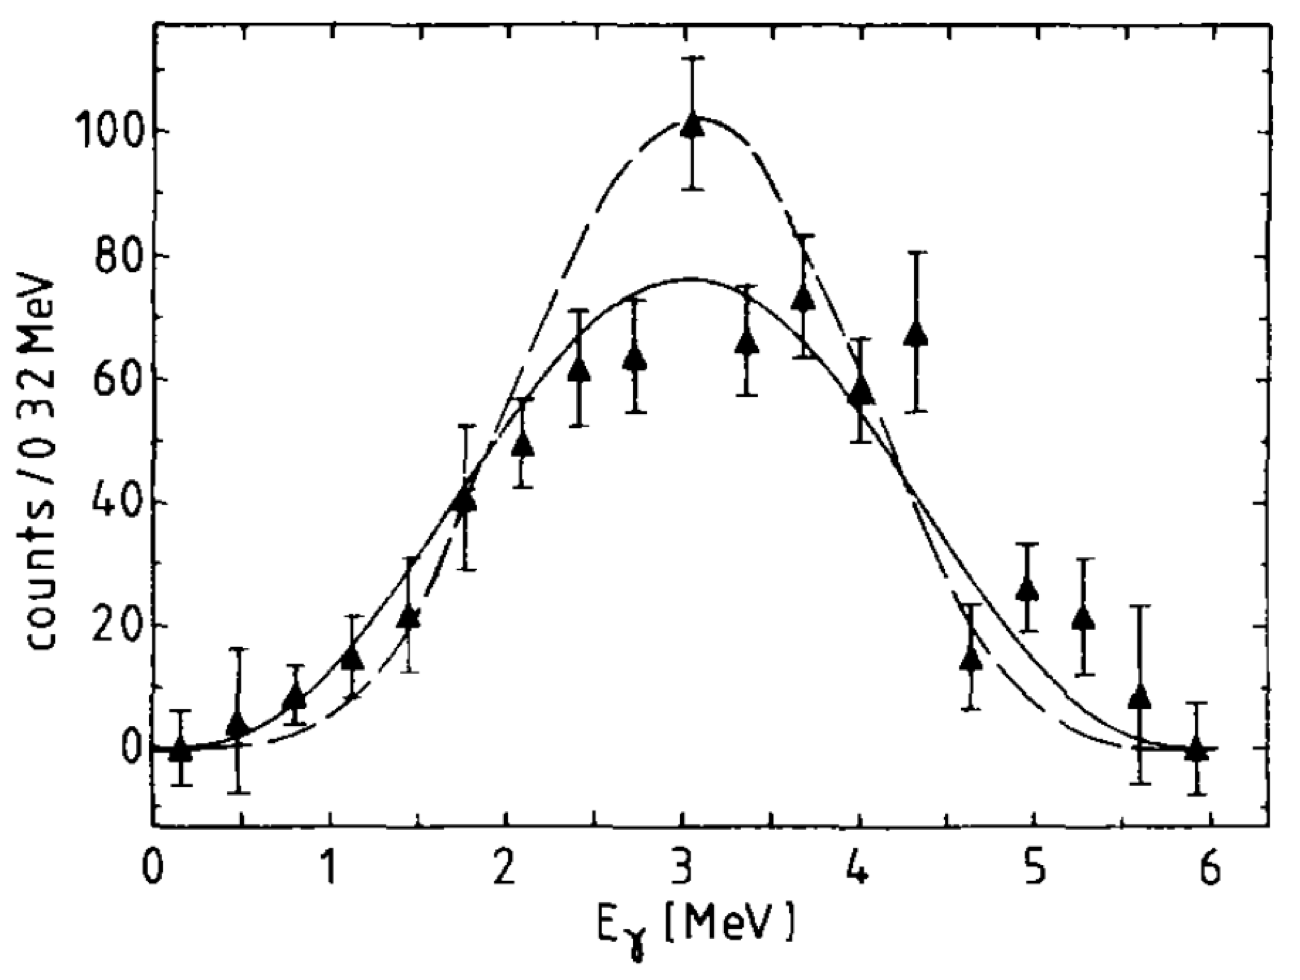
\includegraphics[width=0.95\textwidth]{two_photon_energy_sharing_kramp.png}
    \caption{Energy spectrum for \textit{one} of the two photons for the 6.05 MeV two-photon decay of $^{16}$O. The solid line represents the energy distribution for a pure dipole transition and the dashed line a pure quadrupole transition. Figure from~\cite{kramp_nuclear_1987}.}
    \label{fig:two_photon_energy_sharing_kramp}
\end{figure}
  
According to Ref.~\cite{schirmer_double_1984}, two-photon decay in $^{90}$Zr and $^{40}$Ca occurs not only through two E1 emission but also through equally strong 2M1 emission leading to a linear interference term in the angular correlation function linear with respect to $\cos\theta_{12}$. 
Previous measurements in Ref.~\cite{kramp_nuclear_1987} found the relative branching ratio of 2E2 to 2E1 decays was on the order of $<0.8\%$ with theoretical upper limit of $0.1\%$, motivating the approximation $\alpha_{E2} = 0$.
Equation \ref{eqn:diff_decay_rate_full} becomes 
\begin{equation}
    \frac{d^2\Gamma_{\gamma\gamma}}{d \cos\theta_{12} dE_{\gamma_1}} \propto E_{\gamma_1}^3 E_{\gamma_2}^3 \left( 1 + \frac{4 \alpha_{E1} \chi}{\alpha_{E1}^2 + \chi^2} \cos\theta_{12} +  \cos^2\theta_{12} \right)
\end{equation}
where the angular dependence is decoupled from the energy dependence. 
The expected angular correlation is proportional to
\begin{equation} \label{eqn:angular-distribution}
   W(\theta_{12}) \propto \left( 1 + \frac{4 \alpha_{E1} \chi}{\alpha_{E1}^2 + \chi^2} \cos\theta_{12} +  \cos^2\theta_{12} \right)
\end{equation}
neglecting the linear polarization term present in Ref.~\cite{schirmer_double_1984}.
An example of this distribution is show in~\ref{fig:two_photon_angular_dist} for $^{40}$Ca and $^{90}$Zr.

\begin{figure}[htbp]
    \centering
    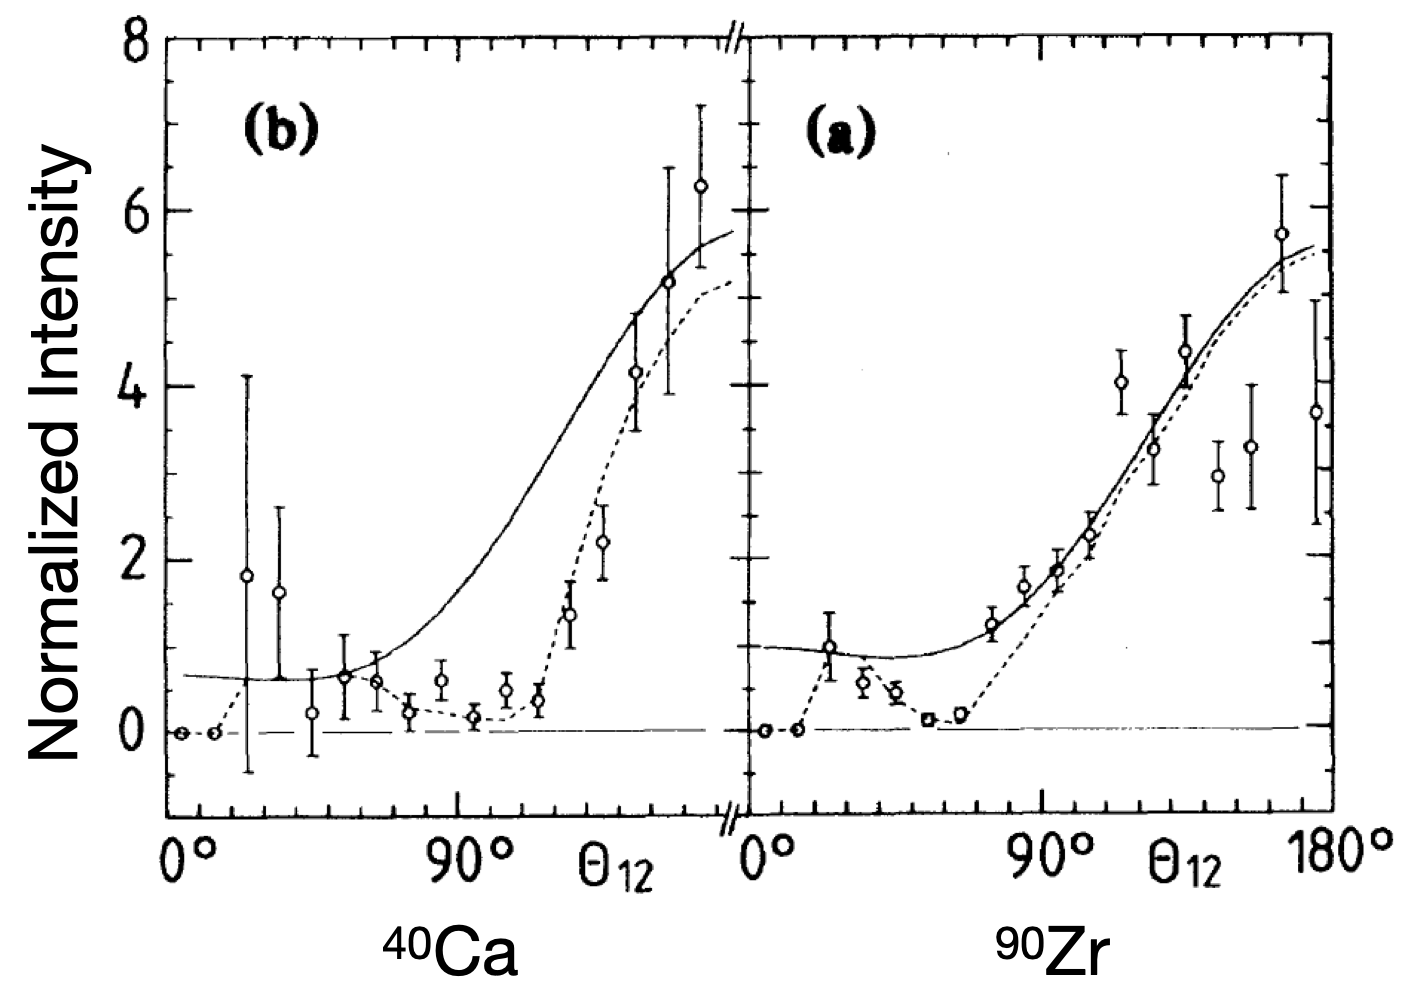
\includegraphics[width=0.95\textwidth]{two_photon_angular_dist.png}
    \caption{Angular distribution of the two-photo decay of $^{40}$Ca and $^{90}$Zr. The dashed lines are the best fit allowing for 2E1 and 2M1 transition and the solid lines represent the calculated correlation if the areas contaminated by Position Annihilation in Flight (PAF) are not excluded. Figure from~\cite{schirmer_double_1984}.}
    \label{fig:two_photon_angular_dist}
\end{figure}

%------------------------------------------
\subsection{Compton-Scattering}
\label{sec:compton_scatter}
%------------------------------------------

Compton scattering takes place when a photon interacts with an atomic electron and is deflected while transferring a portion of its energy to the election. 
This transfer of energy ejects the electron from the nucleus and the $\gamma$-ray is scattered maintaining a fraction of its original energy. 
The energy of the scattered photon, $E^{'}$, can be related to its original energy, $E$, and the scattering angle, $\theta$, via the following:

\begin{equation}
    E^{'} = \frac{E}{1 + \frac{E}{m_e c^2}(1 - \cos(\theta))}
\end{equation}

where $m_e$ is the mass of the electron and $c$ is the speed of light. 

%------------------------------------------
\subsection{Bremsstrahlung Radiation}
\label{sec:bremsstrahlung_radiation}
%------------------------------------------
Bremsstrahlung radiation, also called breaking radiation, is the radiation emitted by charged particles when undergoing acceleration. 
Beta decay electrons interacting with atomic electrons via Coulomb scattering will suffer large deflections and erratic behavior partly due to their relativistic speeds.
In fact the energy transfer is sufficiently large that the incident and deflected electrons become indistinguishable post collision, and the rapid changes in direction and magnitude of velocity necessitates the radiation of electromagnetic energy~\cite{krane_introductory_1987}.
The emitted radiation is called bremsstrahlung radiation. 
The energy loss per unit length for the electons can be written as: 

\begin{align}
    \left(\frac{dE}{dx}\right)_c ={}& \alpha \frac{2 \pi N_0 Z \rho}{m c^2 \beta^2 A} \left[ \ln \frac{T(T + m c^2)^2 \beta^2}{2 I^2 m c^2} + (1 - \beta^2) - (2\sqrt{1 - \beta^2} - 1 + \beta^2) \ln2 + \frac{1}{8}(1 - \sqrt{1 - \beta^2})^2 \right] \\
    \left(\frac{dE}{dx}\right)_r ={}& \alpha \frac{Z^2 N_0 (T + m c^2) \rho}{137 m^2 c^4 A} \left[4 \ln \frac{2(T + m c^2)}{m c^2} - \frac{4}{3} \right] \\
    \alpha = {}& \left(\frac{e^2}{4 \pi \epsilon_0}\right)
\end{align}

where $T$ is the kinetic energy of the electron and the subscripts $c$ and $r$ stand for the energy loss due to collisions and radiation respectively. 

The total energy loss is the sum of the two terms: 

\begin{equation}
    \frac{dE}{dx} = \left(\frac{dE}{dx}\right)_c + \left(\frac{dE}{dx}\right)_r 
\end{equation}

where the radiative term is only valid for relativistic energies, below 1 MeV the radiative losses are negligable.

The ratio of the two terms 

\begin{equation}
    \frac{(dE/dx)_r}{(dE/dx)_c} \approx \frac{T + mc^2}{mc^2} \frac{Z}{1600}
\end{equation}

shows that the radiative term is only significant at high energies and high Z materials~\cite{krane_introductory_1987}.

%------------------------------------------
\end{document}
%------------------------------------------